\documentclass[twoside]{book}

% Packages required by doxygen
\usepackage{fixltx2e}
\usepackage{calc}
\usepackage{doxygen}
\usepackage[export]{adjustbox} % also loads graphicx
\usepackage{graphicx}
\usepackage[utf8]{inputenc}
\usepackage{makeidx}
\usepackage{multicol}
\usepackage{multirow}
\PassOptionsToPackage{warn}{textcomp}
\usepackage{textcomp}
\usepackage[nointegrals]{wasysym}
\usepackage[table]{xcolor}

% Font selection
\usepackage[T1]{fontenc}
\usepackage[scaled=.90]{helvet}
\usepackage{courier}
\usepackage{amssymb}
\usepackage{sectsty}
\renewcommand{\familydefault}{\sfdefault}
\allsectionsfont{%
  \fontseries{bc}\selectfont%
  \color{darkgray}%
}
\renewcommand{\DoxyLabelFont}{%
  \fontseries{bc}\selectfont%
  \color{darkgray}%
}
\newcommand{\+}{\discretionary{\mbox{\scriptsize$\hookleftarrow$}}{}{}}

% Page & text layout
\usepackage{geometry}
\geometry{%
  a4paper,%
  top=2.5cm,%
  bottom=2.5cm,%
  left=2.5cm,%
  right=2.5cm%
}
\tolerance=750
\hfuzz=15pt
\hbadness=750
\setlength{\emergencystretch}{15pt}
\setlength{\parindent}{0cm}
\setlength{\parskip}{3ex plus 2ex minus 2ex}
\makeatletter
\renewcommand{\paragraph}{%
  \@startsection{paragraph}{4}{0ex}{-1.0ex}{1.0ex}{%
    \normalfont\normalsize\bfseries\SS@parafont%
  }%
}
\renewcommand{\subparagraph}{%
  \@startsection{subparagraph}{5}{0ex}{-1.0ex}{1.0ex}{%
    \normalfont\normalsize\bfseries\SS@subparafont%
  }%
}
\makeatother

% Headers & footers
\usepackage{fancyhdr}
\pagestyle{fancyplain}
\fancyhead[LE]{\fancyplain{}{\bfseries\thepage}}
\fancyhead[CE]{\fancyplain{}{}}
\fancyhead[RE]{\fancyplain{}{\bfseries\leftmark}}
\fancyhead[LO]{\fancyplain{}{\bfseries\rightmark}}
\fancyhead[CO]{\fancyplain{}{}}
\fancyhead[RO]{\fancyplain{}{\bfseries\thepage}}
\fancyfoot[LE]{\fancyplain{}{}}
\fancyfoot[CE]{\fancyplain{}{}}
\fancyfoot[RE]{\fancyplain{}{\bfseries\scriptsize Generated by Doxygen }}
\fancyfoot[LO]{\fancyplain{}{\bfseries\scriptsize Generated by Doxygen }}
\fancyfoot[CO]{\fancyplain{}{}}
\fancyfoot[RO]{\fancyplain{}{}}
\renewcommand{\footrulewidth}{0.4pt}
\renewcommand{\chaptermark}[1]{%
  \markboth{#1}{}%
}
\renewcommand{\sectionmark}[1]{%
  \markright{\thesection\ #1}%
}

% Indices & bibliography
\usepackage{natbib}
\usepackage[titles]{tocloft}
\setcounter{tocdepth}{3}
\setcounter{secnumdepth}{5}
\makeindex

% Hyperlinks (required, but should be loaded last)
\usepackage{ifpdf}
\ifpdf
  \usepackage[pdftex,pagebackref=true]{hyperref}
\else
  \usepackage[ps2pdf,pagebackref=true]{hyperref}
\fi
\hypersetup{%
  colorlinks=true,%
  linkcolor=blue,%
  citecolor=blue,%
  unicode%
}

% Custom commands
\newcommand{\clearemptydoublepage}{%
  \newpage{\pagestyle{empty}\cleardoublepage}%
}

\usepackage{caption}
\captionsetup{labelsep=space,justification=centering,font={bf},singlelinecheck=off,skip=4pt,position=top}

%===== C O N T E N T S =====

\begin{document}

% Titlepage & ToC
\hypersetup{pageanchor=false,
             bookmarksnumbered=true,
             pdfencoding=unicode
            }
\pagenumbering{roman}
\begin{titlepage}
\vspace*{7cm}
\begin{center}%
{\Large My Project }\\
\vspace*{1cm}
{\large Generated by Doxygen 1.8.11}\\
\end{center}
\end{titlepage}
\clearemptydoublepage
\tableofcontents
\clearemptydoublepage
\pagenumbering{arabic}
\hypersetup{pageanchor=true}

%--- Begin generated contents ---
\chapter{Module Index}
\section{Modules}
Here is a list of all modules\+:\begin{DoxyCompactList}
\item \contentsline{section}{Figuras\+\_\+\+Planas\+\_\+\+Calc\+Area}{\pageref{group__Figuras__Planas__CalcArea}}{}
\item \contentsline{section}{Figuras\+\_\+\+Espaciais\+\_\+\+Calc\+Area}{\pageref{group__Figuras__Espaciais__CalcArea}}{}
\item \contentsline{section}{Figuras\+\_\+\+Planas\+\_\+\+Inicialização}{\pageref{group__Figuras__Planas__Inicializa_xC3_xA7_xC3_xA3o}}{}
\item \contentsline{section}{Figuras\+\_\+\+Espaciais\+\_\+\+Inicialização}{\pageref{group__Figuras__Espaciais__Inicializa_xC3_xA7_xC3_xA3o}}{}
\end{DoxyCompactList}

\chapter{File Index}
\section{Lista de Arquivos}
Esta é a lista de todos os arquivos documentados e suas respectivas descrições\+:\begin{DoxyCompactList}
\item\contentsline{section}{include/questao\+\_\+1/\hyperlink{area_8h}{area.\+h} \\*Arquivo cabeçalho contendo a definicao das funções que calculam a área das figuras geométricas }{\pageref{area_8h}}{}
\item\contentsline{section}{include/questao\+\_\+1/\hyperlink{calcula_8h}{calcula.\+h} \\*Arquivo cabeçalho contendo a definição das funções que solicitam ao usuário os dados necessários para o cálculo da área, perímetroe volume com a figura geométrica e chamam as funções que realizam essa operação }{\pageref{calcula_8h}}{}
\item\contentsline{section}{include/questao\+\_\+1/\hyperlink{perimetro_8h}{perimetro.\+h} \\*Arquivo cabeçalho contendo a definição das funções que calculam o perímetro de figuras geométricas planas }{\pageref{perimetro_8h}}{}
\item\contentsline{section}{include/questao\+\_\+1/\hyperlink{volume_8h}{volume.\+h} \\*Arquivo cabeçalho contendo a definição das funções que calculam o volume de figuras geométricas espaciais }{\pageref{volume_8h}}{}
\item\contentsline{section}{include/questao\+\_\+2/\hyperlink{fatorial_8h}{fatorial.\+h} \\*Arquivo cabeçalho contendo a definicao das funções que calculam o fatorial do número inteiro inserido pelo usuário }{\pageref{fatorial_8h}}{}
\item\contentsline{section}{include/questao\+\_\+2/\hyperlink{primalidade_8h}{primalidade.\+h} \\*Arquivo cabeçalho contendo a definicao da função recursiva que calcula o maior número primo anterior a um determinado inteiro }{\pageref{primalidade_8h}}{}
\item\contentsline{section}{src/questao\+\_\+1/\hyperlink{area_8cpp}{area.\+cpp} \\*Arquivo corpo contendo a implementação das funções que calculam a área das figuras geométricas }{\pageref{area_8cpp}}{}
\item\contentsline{section}{src/questao\+\_\+1/\hyperlink{perimetro_8cpp}{perimetro.\+cpp} \\*Arquivo contendo contendo a implementação das funções que calculam o perímetro de figuras geométricas planas }{\pageref{perimetro_8cpp}}{}
\item\contentsline{section}{src/questao\+\_\+1/\hyperlink{volume_8cpp}{volume.\+cpp} \\*Arquivo corpo contendo a Implementação das funções que calculam o volume de figuras geométricas espaciais }{\pageref{volume_8cpp}}{}
\item\contentsline{section}{src/questao\+\_\+2/\hyperlink{fatorial_8cpp}{fatorial.\+cpp} \\*Arquivo contendo a implementação da função que calcula o fatorial do número inteiro inserido pelo usuário }{\pageref{fatorial_8cpp}}{}
\item\contentsline{section}{src/questao\+\_\+2/\hyperlink{primalidade_8cpp}{primalidade.\+cpp} \\*Arquivo corpo contendo a implementação da função recursiva que calcula o maior número primo anterior a um determinado inteiro }{\pageref{primalidade_8cpp}}{}
\end{DoxyCompactList}

\chapter{Module Documentation}
\hypertarget{group__Figuras__Planas}{}\section{Figuras\+\_\+\+Planas}
\label{group__Figuras__Planas}\index{Figuras\+\_\+\+Planas@{Figuras\+\_\+\+Planas}}
\subsection*{Functions}
\begin{DoxyCompactItemize}
\item 
void \hyperlink{group__Figuras__Planas_ga8928cef04d4cd48e92adf3569f6d185b}{triangulo} ()\hypertarget{group__Figuras__Planas_ga8928cef04d4cd48e92adf3569f6d185b}{}\label{group__Figuras__Planas_ga8928cef04d4cd48e92adf3569f6d185b}

\begin{DoxyCompactList}\small\item\em Inicializa cálculos para o triângulo. \end{DoxyCompactList}\item 
void \hyperlink{group__Figuras__Planas_gafa7da114af5845aed90385aaad07745f}{retangulo} ()\hypertarget{group__Figuras__Planas_gafa7da114af5845aed90385aaad07745f}{}\label{group__Figuras__Planas_gafa7da114af5845aed90385aaad07745f}

\begin{DoxyCompactList}\small\item\em Inicializa cálculos para o retângulo. \end{DoxyCompactList}\item 
void \hyperlink{group__Figuras__Planas_ga59a769deb5a89245b0b2a7760179708e}{quadrado} ()\hypertarget{group__Figuras__Planas_ga59a769deb5a89245b0b2a7760179708e}{}\label{group__Figuras__Planas_ga59a769deb5a89245b0b2a7760179708e}

\begin{DoxyCompactList}\small\item\em Inicializa cálculos para o quadrado. \end{DoxyCompactList}\item 
void \hyperlink{group__Figuras__Planas_ga28482bc381ce414df86e4fdb9e3e6da5}{circulo} ()\hypertarget{group__Figuras__Planas_ga28482bc381ce414df86e4fdb9e3e6da5}{}\label{group__Figuras__Planas_ga28482bc381ce414df86e4fdb9e3e6da5}

\begin{DoxyCompactList}\small\item\em Inicializa cálculos para o circulo. \end{DoxyCompactList}\end{DoxyCompactItemize}


\subsection{Detailed Description}

\hypertarget{group__Figuras__Espaciais}{}\section{Figuras\+\_\+\+Espaciais}
\label{group__Figuras__Espaciais}\index{Figuras\+\_\+\+Espaciais@{Figuras\+\_\+\+Espaciais}}
\subsection*{Functions}
\begin{DoxyCompactItemize}
\item 
void \hyperlink{group__Figuras__Espaciais_gae3945922f925bc3d1fd95c5dc4ff6987}{piramide} ()\hypertarget{group__Figuras__Espaciais_gae3945922f925bc3d1fd95c5dc4ff6987}{}\label{group__Figuras__Espaciais_gae3945922f925bc3d1fd95c5dc4ff6987}

\begin{DoxyCompactList}\small\item\em Inicializa cálculos para a piramide. \end{DoxyCompactList}\item 
void \hyperlink{group__Figuras__Espaciais_gaf0b7d023166ce6902197d4082a66ad03}{cubo} ()\hypertarget{group__Figuras__Espaciais_gaf0b7d023166ce6902197d4082a66ad03}{}\label{group__Figuras__Espaciais_gaf0b7d023166ce6902197d4082a66ad03}

\begin{DoxyCompactList}\small\item\em Inicializa cálculos para o cubo. \end{DoxyCompactList}\item 
void \hyperlink{group__Figuras__Espaciais_gaf5c3350f35c2d9ae97c0243b7aeac39e}{paralelepipedo} ()\hypertarget{group__Figuras__Espaciais_gaf5c3350f35c2d9ae97c0243b7aeac39e}{}\label{group__Figuras__Espaciais_gaf5c3350f35c2d9ae97c0243b7aeac39e}

\begin{DoxyCompactList}\small\item\em Inicializa cálculos para o paralelepípedo. \end{DoxyCompactList}\item 
void \hyperlink{group__Figuras__Espaciais_ga947bf2f326598c591bbdbf77a0280266}{esfera} ()\hypertarget{group__Figuras__Espaciais_ga947bf2f326598c591bbdbf77a0280266}{}\label{group__Figuras__Espaciais_ga947bf2f326598c591bbdbf77a0280266}

\begin{DoxyCompactList}\small\item\em Inicializa cálculos para a esfera. \end{DoxyCompactList}\end{DoxyCompactItemize}


\subsection{Detailed Description}

\chapter{File Documentation}
\hypertarget{area_8h}{}\section{Referência do Arquivo include/questao\+\_\+1/area.h}
\label{area_8h}\index{include/questao\+\_\+1/area.\+h@{include/questao\+\_\+1/area.\+h}}


Arquivo cabeçalho contendo a definicao das funções que calculam a área das figuras geométricas.  


Este grafo mostra quais arquivos estão direta ou indiretamente relacionados com este arquivo\+:
\nopagebreak
\begin{figure}[H]
\begin{center}
\leavevmode
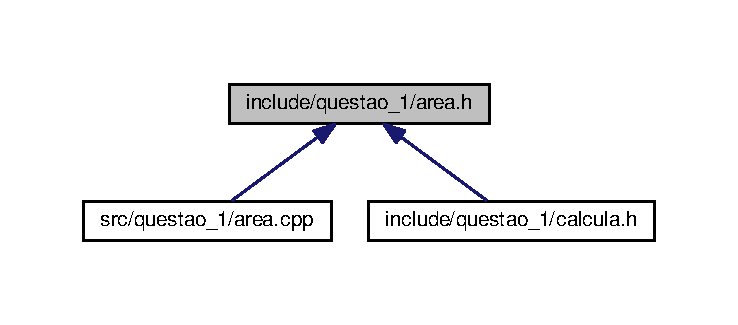
\includegraphics[width=350pt]{area_8h__dep__incl}
\end{center}
\end{figure}
\subsection*{Funções}
\begin{DoxyCompactItemize}
\item 
float \hyperlink{group__Figuras__Planas__CalcArea_gad3dd4559c961d21265a1fe46e7d5c3cc}{triangulo\+Area} (float \&base)
\begin{DoxyCompactList}\small\item\em Função que calcula o valor da área do triangulo. \end{DoxyCompactList}\item 
float \hyperlink{group__Figuras__Planas__CalcArea_gaadec7ea7b857fb93862af9da30f4b896}{retangulo\+Area} (float \&base, float \&altura)
\begin{DoxyCompactList}\small\item\em Função que calcula o valor da área do retângulo. \end{DoxyCompactList}\item 
float \hyperlink{group__Figuras__Planas__CalcArea_gac85a6a6234680349b5b8329d4333567e}{quadrado\+Area} (float \&lado)
\begin{DoxyCompactList}\small\item\em Função que calcula o valor da área do quadrado. \end{DoxyCompactList}\item 
float \hyperlink{group__Figuras__Planas__CalcArea_gac50529a5e8458336df0f0e2329e49833}{circulo\+Area} (float \&raio)
\begin{DoxyCompactList}\small\item\em Função que calcula o valor da área do círculo. \end{DoxyCompactList}\item 
float \hyperlink{group__Figuras__Espaciais__CalcArea_ga10226ad45447d70353626a01897d1b06}{area\+Piramide} (float \&base, float \&altura)
\begin{DoxyCompactList}\small\item\em Função que calcula o valor da área da pirâmide. \end{DoxyCompactList}\item 
float \hyperlink{group__Figuras__Espaciais__CalcArea_gab519a0d997044a93085abaaaf6270ab5}{area\+Cubo} (float \&aresta)
\begin{DoxyCompactList}\small\item\em Função que calcula o valor da área do cubo. \end{DoxyCompactList}\item 
float \hyperlink{group__Figuras__Espaciais__CalcArea_gaff7dfecfa742b07c8e8e243325d95117}{area\+Paralelepipedo} (float \&aresta1, float \&aresta2, float \&aresta3)
\begin{DoxyCompactList}\small\item\em Função que calcula o valor da área do paralelepípedo. \end{DoxyCompactList}\item 
float \hyperlink{group__Figuras__Espaciais__CalcArea_ga2d0b18f7e5391dd6a8bff93bb679171a}{area\+Esfera} (float \&raio)
\begin{DoxyCompactList}\small\item\em Função que calcula o valor da área da esfera. \end{DoxyCompactList}\end{DoxyCompactItemize}


\subsection{Descrição Detalhada}
Arquivo cabeçalho contendo a definicao das funções que calculam a área das figuras geométricas. 

\begin{DoxyAuthor}{Autor}
Ariel Oliveira (\href{mailto:ariel.oliveira01@gmail.com}{\tt ariel.\+oliveira01@gmail.\+com}) 
\end{DoxyAuthor}
\begin{DoxySince}{Desde}
10/08/2017 
\end{DoxySince}
\begin{DoxyDate}{Data}
15/08/2017 
\end{DoxyDate}

\hypertarget{calcarea_8h}{}\section{include/calcarea.h File Reference}
\label{calcarea_8h}\index{include/calcarea.\+h@{include/calcarea.\+h}}


Arquivo cabeçalho contendo a definição das funções que solicitam ao usuário os dados necessários para o cálculo da área com a figura geométrica e chamam as funções que realizam essa operação.  


{\ttfamily \#include \char`\"{}area.\+h\char`\"{}}\\*
Include dependency graph for calcarea.\+h\+:
\nopagebreak
\begin{figure}[H]
\begin{center}
\leavevmode
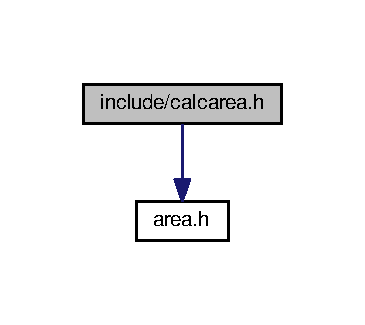
\includegraphics[width=175pt]{calcarea_8h__incl}
\end{center}
\end{figure}
This graph shows which files directly or indirectly include this file\+:
\nopagebreak
\begin{figure}[H]
\begin{center}
\leavevmode
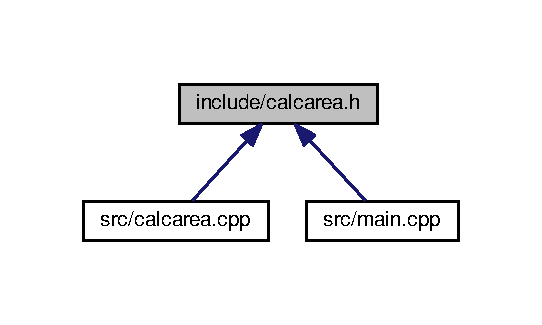
\includegraphics[width=260pt]{calcarea_8h__dep__incl}
\end{center}
\end{figure}
\subsection*{Functions}
\begin{DoxyCompactItemize}
\item 
void \hyperlink{group__Figuras__Planas__Imprime__Resultado_gac0d6d9fb68ed0e43ad9780f0c86cac51}{calc\+Area\+Triangulo} (float \&base)
\begin{DoxyCompactList}\small\item\em Função que imprime o valor da área do triângulo. \end{DoxyCompactList}\item 
void \hyperlink{group__Figuras__Planas__Imprime__Resultado_ga1091311f26d5adb888dae930fc1ec7d6}{calc\+Area\+Retangulo} (float \&base, float \&altura)
\begin{DoxyCompactList}\small\item\em Função que imprime o valor da área do retângulo. \end{DoxyCompactList}\item 
void \hyperlink{group__Figuras__Planas__Imprime__Resultado_gaabb19ec0d92baa5524a15b463f854158}{calc\+Area\+Quadrado} (float \&base)
\begin{DoxyCompactList}\small\item\em Função que imprime o valor da área do quadrado. \end{DoxyCompactList}\item 
void \hyperlink{group__Figuras__Planas__Imprime__Resultado_gafc4965f40035f915dd29f3a2fe680339}{calc\+Area\+Circulo} (float \&raio)
\begin{DoxyCompactList}\small\item\em Função que imprime o valor da área do círculo. \end{DoxyCompactList}\item 
void \hyperlink{group__Figuras__Espaciais__Imprime__Resultado_gae484b707bcee07b0c5580440923326aa}{calc\+Area\+Piramide} (float \&base, float \&altura)
\begin{DoxyCompactList}\small\item\em Função que imprime o valor da área da pirâmide. \end{DoxyCompactList}\item 
void \hyperlink{group__Figuras__Espaciais__Imprime__Resultado_ga54aa7364c2caf59fa3d1b1b303901050}{calc\+Area\+Cubo} (float \&aresta)
\begin{DoxyCompactList}\small\item\em Função que imprime o valor da área do círculo. \end{DoxyCompactList}\item 
void \hyperlink{group__Figuras__Espaciais__Imprime__Resultado_ga153e7a3b91362f17f7f22919dde85ebc}{calc\+Area\+Paralelepipedo} (float \&aresta1, float \&aresta2, float \&aresta3)
\begin{DoxyCompactList}\small\item\em Função que imprime o valor da área do paralelepípedo. \end{DoxyCompactList}\item 
void \hyperlink{group__Figuras__Espaciais__Imprime__Resultado_ga3a49e8821532ada5f803c815f8d99825}{calc\+Area\+Esfera} (float \&raio)
\begin{DoxyCompactList}\small\item\em Função que imprime o valor da área do círculo. \end{DoxyCompactList}\end{DoxyCompactItemize}


\subsection{Detailed Description}
Arquivo cabeçalho contendo a definição das funções que solicitam ao usuário os dados necessários para o cálculo da área com a figura geométrica e chamam as funções que realizam essa operação. 

\begin{DoxyAuthor}{Author}
Gabriel Barbosa (\href{mailto:gbsbarbosa.gb@gmail.com}{\tt gbsbarbosa.\+gb@gmail.\+com}) 

Ariel Oliveira (\href{mailto:ariel.oliveira01@gmail.com}{\tt ariel.\+oliveira01@gmail.\+com}) 
\end{DoxyAuthor}
\begin{DoxySince}{Since}
09/03/2017 
\end{DoxySince}
\begin{DoxyDate}{Date}
12/03/2017 
\end{DoxyDate}
\begin{DoxySeeAlso}{See also}
\hyperlink{area_8h}{area.\+h} 
\end{DoxySeeAlso}

\hypertarget{calcperimetro_8h}{}\section{include/calcperimetro.h File Reference}
\label{calcperimetro_8h}\index{include/calcperimetro.\+h@{include/calcperimetro.\+h}}


Arquivo cabecalho contendo a definicao das funções que solicitam ao usuário os dados necessários ao cálculo do perimetro da figura geométrica e chamam as funções que realizam essa operação.  


{\ttfamily \#include \char`\"{}perimetro.\+h\char`\"{}}\\*
Include dependency graph for calcperimetro.\+h\+:
\nopagebreak
\begin{figure}[H]
\begin{center}
\leavevmode
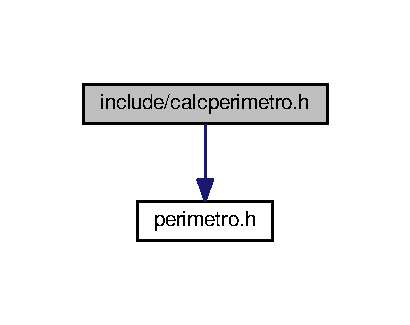
\includegraphics[width=197pt]{calcperimetro_8h__incl}
\end{center}
\end{figure}
This graph shows which files directly or indirectly include this file\+:
\nopagebreak
\begin{figure}[H]
\begin{center}
\leavevmode
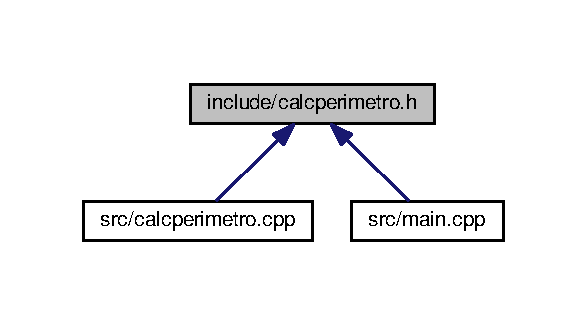
\includegraphics[width=282pt]{calcperimetro_8h__dep__incl}
\end{center}
\end{figure}
\subsection*{Functions}
\begin{DoxyCompactItemize}
\item 
void \hyperlink{calcperimetro_8h_ae49d939eed738e7168cd0efd8b40c09c}{calc\+Perimetro\+Triangulo} (float \&base)
\begin{DoxyCompactList}\small\item\em Funcao que imprime o valor do perimetro do triangulo. \end{DoxyCompactList}\item 
void \hyperlink{calcperimetro_8h_ab29565d71c21097aef26e73d36b9c8a6}{calc\+Perimetro\+Retangulo} (float \&base, float \&altura)
\begin{DoxyCompactList}\small\item\em Funcao que imprime o valor do perimetro do retangulo. \end{DoxyCompactList}\item 
void \hyperlink{calcperimetro_8h_acaef8cc731e8f6564e033dadcbefa04f}{calc\+Perimetro\+Quadrado} (float \&base)
\begin{DoxyCompactList}\small\item\em Funcao que imprime o valor do perimetro do quadrado. \end{DoxyCompactList}\item 
void \hyperlink{calcperimetro_8h_a6f116584d476bf2a78f83cb668e1f25b}{calc\+Perimetro\+Circulo} (float \&raio)
\begin{DoxyCompactList}\small\item\em Funcao que imprime o valor do perimetro do circulo. \end{DoxyCompactList}\end{DoxyCompactItemize}


\subsection{Detailed Description}
Arquivo cabecalho contendo a definicao das funções que solicitam ao usuário os dados necessários ao cálculo do perimetro da figura geométrica e chamam as funções que realizam essa operação. 

\begin{DoxyAuthor}{Author}
Gabriel Barbosa (\href{mailto:gbsbarbosa.gb@gmail.com}{\tt gbsbarbosa.\+gb@gmail.\+com}) 

Ariel Oliveira (\href{mailto:ariel.oliveira01@gmail.com}{\tt ariel.\+oliveira01@gmail.\+com}) 
\end{DoxyAuthor}
\begin{DoxySince}{Since}
12/03/2017 
\end{DoxySince}
\begin{DoxyDate}{Date}
21/03/2017 
\end{DoxyDate}
\begin{DoxySeeAlso}{See also}
\hyperlink{perimetro_8h}{perimetro.\+h} 
\end{DoxySeeAlso}


\subsection{Function Documentation}
\index{calcperimetro.\+h@{calcperimetro.\+h}!calc\+Perimetro\+Circulo@{calc\+Perimetro\+Circulo}}
\index{calc\+Perimetro\+Circulo@{calc\+Perimetro\+Circulo}!calcperimetro.\+h@{calcperimetro.\+h}}
\subsubsection[{\texorpdfstring{calc\+Perimetro\+Circulo(float \&raio)}{calcPerimetroCirculo(float &raio)}}]{\setlength{\rightskip}{0pt plus 5cm}void calc\+Perimetro\+Circulo (
\begin{DoxyParamCaption}
\item[{float \&}]{raio}
\end{DoxyParamCaption}
)}\hypertarget{calcperimetro_8h_a6f116584d476bf2a78f83cb668e1f25b}{}\label{calcperimetro_8h_a6f116584d476bf2a78f83cb668e1f25b}


Funcao que imprime o valor do perimetro do circulo. 


\begin{DoxyParams}{Parameters}
{\em base} & B\+A\+SE valor da base do circulo \\
\hline
\end{DoxyParams}
\index{calcperimetro.\+h@{calcperimetro.\+h}!calc\+Perimetro\+Quadrado@{calc\+Perimetro\+Quadrado}}
\index{calc\+Perimetro\+Quadrado@{calc\+Perimetro\+Quadrado}!calcperimetro.\+h@{calcperimetro.\+h}}
\subsubsection[{\texorpdfstring{calc\+Perimetro\+Quadrado(float \&base)}{calcPerimetroQuadrado(float &base)}}]{\setlength{\rightskip}{0pt plus 5cm}void calc\+Perimetro\+Quadrado (
\begin{DoxyParamCaption}
\item[{float \&}]{base}
\end{DoxyParamCaption}
)}\hypertarget{calcperimetro_8h_acaef8cc731e8f6564e033dadcbefa04f}{}\label{calcperimetro_8h_acaef8cc731e8f6564e033dadcbefa04f}


Funcao que imprime o valor do perimetro do quadrado. 


\begin{DoxyParams}{Parameters}
{\em base} & B\+A\+SE valor da base do quadrado \\
\hline
\end{DoxyParams}
\index{calcperimetro.\+h@{calcperimetro.\+h}!calc\+Perimetro\+Retangulo@{calc\+Perimetro\+Retangulo}}
\index{calc\+Perimetro\+Retangulo@{calc\+Perimetro\+Retangulo}!calcperimetro.\+h@{calcperimetro.\+h}}
\subsubsection[{\texorpdfstring{calc\+Perimetro\+Retangulo(float \&base, float \&altura)}{calcPerimetroRetangulo(float &base, float &altura)}}]{\setlength{\rightskip}{0pt plus 5cm}void calc\+Perimetro\+Retangulo (
\begin{DoxyParamCaption}
\item[{float \&}]{base, }
\item[{float \&}]{altura}
\end{DoxyParamCaption}
)}\hypertarget{calcperimetro_8h_ab29565d71c21097aef26e73d36b9c8a6}{}\label{calcperimetro_8h_ab29565d71c21097aef26e73d36b9c8a6}


Funcao que imprime o valor do perimetro do retangulo. 


\begin{DoxyParams}{Parameters}
{\em base} & B\+A\+SE valor da base do retangulo \\
\hline
{\em altura} & A\+L\+T\+U\+RA valor da altura do retangulo \\
\hline
\end{DoxyParams}
\index{calcperimetro.\+h@{calcperimetro.\+h}!calc\+Perimetro\+Triangulo@{calc\+Perimetro\+Triangulo}}
\index{calc\+Perimetro\+Triangulo@{calc\+Perimetro\+Triangulo}!calcperimetro.\+h@{calcperimetro.\+h}}
\subsubsection[{\texorpdfstring{calc\+Perimetro\+Triangulo(float \&base)}{calcPerimetroTriangulo(float &base)}}]{\setlength{\rightskip}{0pt plus 5cm}void calc\+Perimetro\+Triangulo (
\begin{DoxyParamCaption}
\item[{float \&}]{base}
\end{DoxyParamCaption}
)}\hypertarget{calcperimetro_8h_ae49d939eed738e7168cd0efd8b40c09c}{}\label{calcperimetro_8h_ae49d939eed738e7168cd0efd8b40c09c}


Funcao que imprime o valor do perimetro do triangulo. 


\begin{DoxyParams}{Parameters}
{\em base} & B\+A\+SE valor da base do triangulo \\
\hline
\end{DoxyParams}

\hypertarget{calcvolume_8h}{}\section{include/calcvolume.h File Reference}
\label{calcvolume_8h}\index{include/calcvolume.\+h@{include/calcvolume.\+h}}


Arquivo cabeçalho contendo a definição das funções que solicitam ao usuário os dados necessários para o cálculo do volume com a figura geométrica e chamam as funções que realizam essa operação.  


{\ttfamily \#include \char`\"{}volume.\+h\char`\"{}}\\*
Include dependency graph for calcvolume.\+h\+:
\nopagebreak
\begin{figure}[H]
\begin{center}
\leavevmode
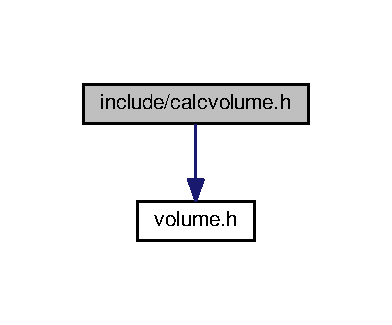
\includegraphics[width=188pt]{calcvolume_8h__incl}
\end{center}
\end{figure}
This graph shows which files directly or indirectly include this file\+:
\nopagebreak
\begin{figure}[H]
\begin{center}
\leavevmode
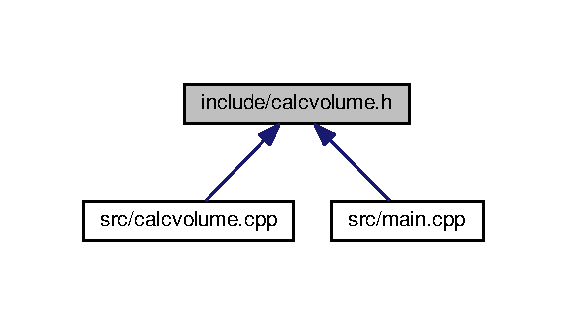
\includegraphics[width=272pt]{calcvolume_8h__dep__incl}
\end{center}
\end{figure}
\subsection*{Functions}
\begin{DoxyCompactItemize}
\item 
void \hyperlink{calcvolume_8h_aa5acf0ff0f4eb8061d1b86334d2838de}{calc\+Volume\+Piramide} (float \&base, float \&altura)
\begin{DoxyCompactList}\small\item\em Função que imprime o valor do volume da piramide. \end{DoxyCompactList}\item 
void \hyperlink{calcvolume_8h_af35d29634faa808e187b6635ac6e1fb9}{calc\+Volume\+Cubo} (float \&aresta)
\begin{DoxyCompactList}\small\item\em Função que imprime o valor do volume do cubo. \end{DoxyCompactList}\item 
void \hyperlink{calcvolume_8h_a994d3c26012b734a4cbabf0ce0c7b75b}{calc\+Volume\+Paralelepipedo} (float \&aresta1, float \&aresta2, float \&aresta3)
\begin{DoxyCompactList}\small\item\em Função que imprime o valor do volume do paralelepípedo. \end{DoxyCompactList}\item 
void \hyperlink{calcvolume_8h_addef3fdcde1a2b12007610961caffae5}{calc\+Volume\+Esfera} (float \&raio)
\begin{DoxyCompactList}\small\item\em Função que imprime o valor do volume da esfera. \end{DoxyCompactList}\end{DoxyCompactItemize}


\subsection{Detailed Description}
Arquivo cabeçalho contendo a definição das funções que solicitam ao usuário os dados necessários para o cálculo do volume com a figura geométrica e chamam as funções que realizam essa operação. 

\begin{DoxyAuthor}{Author}
Gabriel Barbosa (\href{mailto:gbsbarbosa.gb@gmail.com}{\tt gbsbarbosa.\+gb@gmail.\+com}) 

Ariel Oliveira (\href{mailto:ariel.oliveira01@gmail.com}{\tt ariel.\+oliveira01@gmail.\+com}) 
\end{DoxyAuthor}
\begin{DoxySince}{Since}
09/03/2017 
\end{DoxySince}
\begin{DoxyDate}{Date}
12/03/2017 
\end{DoxyDate}
\begin{DoxySeeAlso}{See also}
\hyperlink{volume_8h}{volume.\+h} 
\end{DoxySeeAlso}


\subsection{Function Documentation}
\index{calcvolume.\+h@{calcvolume.\+h}!calc\+Volume\+Cubo@{calc\+Volume\+Cubo}}
\index{calc\+Volume\+Cubo@{calc\+Volume\+Cubo}!calcvolume.\+h@{calcvolume.\+h}}
\subsubsection[{\texorpdfstring{calc\+Volume\+Cubo(float \&aresta)}{calcVolumeCubo(float &aresta)}}]{\setlength{\rightskip}{0pt plus 5cm}void calc\+Volume\+Cubo (
\begin{DoxyParamCaption}
\item[{float \&}]{aresta}
\end{DoxyParamCaption}
)}\hypertarget{calcvolume_8h_af35d29634faa808e187b6635ac6e1fb9}{}\label{calcvolume_8h_af35d29634faa808e187b6635ac6e1fb9}


Função que imprime o valor do volume do cubo. 


\begin{DoxyParams}{Parameters}
{\em aresta} & A\+R\+E\+S\+TA valor da aresta do cubo \\
\hline
\end{DoxyParams}
\index{calcvolume.\+h@{calcvolume.\+h}!calc\+Volume\+Esfera@{calc\+Volume\+Esfera}}
\index{calc\+Volume\+Esfera@{calc\+Volume\+Esfera}!calcvolume.\+h@{calcvolume.\+h}}
\subsubsection[{\texorpdfstring{calc\+Volume\+Esfera(float \&raio)}{calcVolumeEsfera(float &raio)}}]{\setlength{\rightskip}{0pt plus 5cm}void calc\+Volume\+Esfera (
\begin{DoxyParamCaption}
\item[{float \&}]{raio}
\end{DoxyParamCaption}
)}\hypertarget{calcvolume_8h_addef3fdcde1a2b12007610961caffae5}{}\label{calcvolume_8h_addef3fdcde1a2b12007610961caffae5}


Função que imprime o valor do volume da esfera. 


\begin{DoxyParams}{Parameters}
{\em raio} & R\+A\+IO valor do raio do cubo \\
\hline
\end{DoxyParams}
\index{calcvolume.\+h@{calcvolume.\+h}!calc\+Volume\+Paralelepipedo@{calc\+Volume\+Paralelepipedo}}
\index{calc\+Volume\+Paralelepipedo@{calc\+Volume\+Paralelepipedo}!calcvolume.\+h@{calcvolume.\+h}}
\subsubsection[{\texorpdfstring{calc\+Volume\+Paralelepipedo(float \&aresta1, float \&aresta2, float \&aresta3)}{calcVolumeParalelepipedo(float &aresta1, float &aresta2, float &aresta3)}}]{\setlength{\rightskip}{0pt plus 5cm}void calc\+Volume\+Paralelepipedo (
\begin{DoxyParamCaption}
\item[{float \&}]{aresta1, }
\item[{float \&}]{aresta2, }
\item[{float \&}]{aresta3}
\end{DoxyParamCaption}
)}\hypertarget{calcvolume_8h_a994d3c26012b734a4cbabf0ce0c7b75b}{}\label{calcvolume_8h_a994d3c26012b734a4cbabf0ce0c7b75b}


Função que imprime o valor do volume do paralelepípedo. 


\begin{DoxyParams}{Parameters}
{\em aresta1} & A\+R\+E\+S\+T\+A1 valor da aresta \#1 do paralelepípedo \\
\hline
{\em aresta2} & A\+R\+E\+S\+T\+A2 valor da aresta \#2 do paralelepípedo \\
\hline
{\em aresta3} & A\+R\+E\+S\+T\+A3 valor da aresta \#3 do paralelepípedo \\
\hline
\end{DoxyParams}
\index{calcvolume.\+h@{calcvolume.\+h}!calc\+Volume\+Piramide@{calc\+Volume\+Piramide}}
\index{calc\+Volume\+Piramide@{calc\+Volume\+Piramide}!calcvolume.\+h@{calcvolume.\+h}}
\subsubsection[{\texorpdfstring{calc\+Volume\+Piramide(float \&base, float \&altura)}{calcVolumePiramide(float &base, float &altura)}}]{\setlength{\rightskip}{0pt plus 5cm}void calc\+Volume\+Piramide (
\begin{DoxyParamCaption}
\item[{float \&}]{base, }
\item[{float \&}]{altura}
\end{DoxyParamCaption}
)}\hypertarget{calcvolume_8h_aa5acf0ff0f4eb8061d1b86334d2838de}{}\label{calcvolume_8h_aa5acf0ff0f4eb8061d1b86334d2838de}


Função que imprime o valor do volume da piramide. 


\begin{DoxyParams}{Parameters}
{\em base} & B\+A\+SE valor da base da piramide \\
\hline
{\em altura} & A\+L\+T\+U\+RA valor da altura da piramide\\
\hline
{\em base} & B\+A\+SE valor da base da piramide \\
\hline
{\em altura} & A\+L\+T\+U\+RA valor da altura da piramide Funcao que imprime o valor do volume da piramide \\
\hline
{\em base} & B\+A\+SE valor da base da piramide \\
\hline
{\em altura} & A\+L\+T\+U\+RA valor da altura da piramide \\
\hline
\end{DoxyParams}

\hypertarget{perimetro_8h}{}\section{include/perimetro.h File Reference}
\label{perimetro_8h}\index{include/perimetro.\+h@{include/perimetro.\+h}}


Arquivo cabeçalho contendo a definição das funções que calculam o perímetro de figuras geométricas planas.  


This graph shows which files directly or indirectly include this file\+:
\nopagebreak
\begin{figure}[H]
\begin{center}
\leavevmode
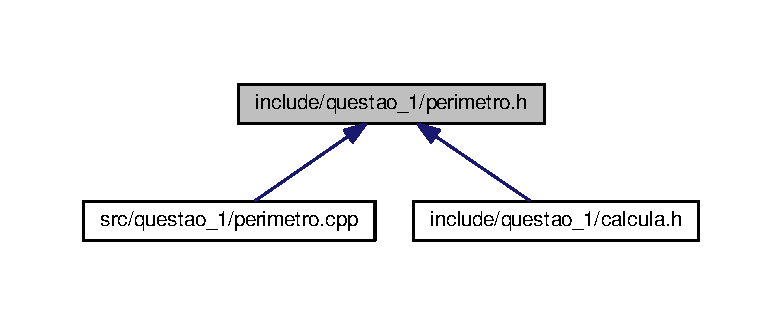
\includegraphics[width=341pt]{perimetro_8h__dep__incl}
\end{center}
\end{figure}
\subsection*{Functions}
\begin{DoxyCompactItemize}
\item 
float \hyperlink{group__Calc__Perimetro_ga76a18caf86cad87741930b6b73a28e6d}{triangulo\+Perimetro} (float \&base)
\begin{DoxyCompactList}\small\item\em Função que calcula o valor do perímetro do triângulo. \end{DoxyCompactList}\item 
float \hyperlink{group__Calc__Perimetro_ga818dc286a8e9892293bddf8c2c4611dd}{retangulo\+Perimetro} (float \&base, float \&altura)
\begin{DoxyCompactList}\small\item\em Função que calcula o valor do perímetro do retângulo. \end{DoxyCompactList}\item 
float \hyperlink{group__Calc__Perimetro_ga262504d9854cd41bc2519504de0531ca}{quadrado\+Perimetro} (float \&base)
\begin{DoxyCompactList}\small\item\em Função que calcula o valor do perímetro do quadrado. \end{DoxyCompactList}\item 
float \hyperlink{group__Calc__Perimetro_gabf774992f344a535b77e941cabb7e2f0}{circulo\+Perimetro} (float \&raio)
\begin{DoxyCompactList}\small\item\em Função que calcula o valor do perímetro do círculo. \end{DoxyCompactList}\end{DoxyCompactItemize}


\subsection{Detailed Description}
Arquivo cabeçalho contendo a definição das funções que calculam o perímetro de figuras geométricas planas. 

\begin{DoxyAuthor}{Author}
Gabriel Barbosa (\href{mailto:gbsbarbosa.gb@gmail.com}{\tt gbsbarbosa.\+gb@gmail.\+com}) 

Ariel Oliveira (\href{mailto:ariel.oliveira01@gmail.com}{\tt ariel.\+oliveira01@gmail.\+com}) 
\end{DoxyAuthor}
\begin{DoxySince}{Since}
12/03/2017 
\end{DoxySince}
\begin{DoxyDate}{Date}
21/03/2017 
\end{DoxyDate}

\hypertarget{volume_8h}{}\section{Referência do Arquivo include/questao\+\_\+1/volume.h}
\label{volume_8h}\index{include/questao\+\_\+1/volume.\+h@{include/questao\+\_\+1/volume.\+h}}


Arquivo cabeçalho contendo a definição das funções que calculam o volume de figuras geométricas espaciais.  


Este grafo mostra quais arquivos estão direta ou indiretamente relacionados com este arquivo\+:
\nopagebreak
\begin{figure}[H]
\begin{center}
\leavevmode
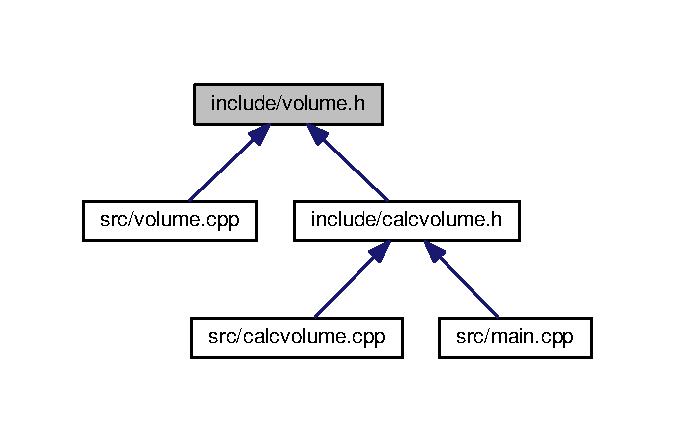
\includegraphics[width=350pt]{volume_8h__dep__incl}
\end{center}
\end{figure}
\subsection*{Funções}
\begin{DoxyCompactItemize}
\item 
float \hyperlink{group__Calc__Volume_ga4a36098bad980501fa8e5d0229309098}{volume\+Piramide} (float \&base, float \&altura)
\begin{DoxyCompactList}\small\item\em Função que calcula o valor do volume da pirâmide. \end{DoxyCompactList}\item 
float \hyperlink{group__Calc__Volume_ga43aaef1a010e2ccbe7e5389aa5be3366}{volume\+Cubo} (float \&aresta)
\begin{DoxyCompactList}\small\item\em Função que calcula o valor do volume do cubo. \end{DoxyCompactList}\item 
float \hyperlink{group__Calc__Volume_gadf67b3277ecfcf3e6e225e1f66e30a23}{volume\+Paralelepipedo} (float \&aresta1, float \&aresta2, float \&aresta3)
\begin{DoxyCompactList}\small\item\em Função que calcula o valor do volume do paralelepípedo. \end{DoxyCompactList}\item 
float \hyperlink{group__Calc__Volume_gaf649387c42d43094c7c81e2f26face42}{volume\+Esfera} (float \&raio)
\begin{DoxyCompactList}\small\item\em Função que calcula o valor do volume da esfera. \end{DoxyCompactList}\end{DoxyCompactItemize}


\subsection{Descrição Detalhada}
Arquivo cabeçalho contendo a definição das funções que calculam o volume de figuras geométricas espaciais. 

\begin{DoxyAuthor}{Autor}
Ariel Oliveira (\href{mailto:ariel.oliveira01@gmail.com}{\tt ariel.\+oliveira01@gmail.\+com}) 
\end{DoxyAuthor}
\begin{DoxySince}{Desde}
10/08/2017 
\end{DoxySince}
\begin{DoxyDate}{Data}
15/08/2017 
\end{DoxyDate}

\hypertarget{area_8cpp}{}\section{src/area.cpp File Reference}
\label{area_8cpp}\index{src/area.\+cpp@{src/area.\+cpp}}


Arquivo cabeçalho contendo a definição das funções que calculam a área das figuras geométricas.  


{\ttfamily \#include $<$cmath$>$}\\*
{\ttfamily \#include \char`\"{}area.\+h\char`\"{}}\\*
Include dependency graph for area.\+cpp\+:
% FIG 0
\subsection*{Macros}
\begin{DoxyCompactItemize}
\item 
\#define {\bfseries PI}~3.\+1415\hypertarget{area_8cpp_a598a3330b3c21701223ee0ca14316eca}{}\label{area_8cpp_a598a3330b3c21701223ee0ca14316eca}

\item 
\#define {\bfseries pitagoras}(a,  b)~(pow(a,2) -\/ pow(b,2))\hypertarget{area_8cpp_a4544bdcd1e3ebe0263d82aad9efa4901}{}\label{area_8cpp_a4544bdcd1e3ebe0263d82aad9efa4901}

\end{DoxyCompactItemize}
\subsection*{Functions}
\begin{DoxyCompactItemize}
\item 
float \hyperlink{area_8cpp_ad3dd4559c961d21265a1fe46e7d5c3cc}{triangulo\+Area} (float \&base)
\begin{DoxyCompactList}\small\item\em Função que calcula o valor da área do triângulo. \end{DoxyCompactList}\item 
float \hyperlink{area_8cpp_aadec7ea7b857fb93862af9da30f4b896}{retangulo\+Area} (float \&base, float \&altura)
\begin{DoxyCompactList}\small\item\em Função que calcula o valor da área do retângulo. \end{DoxyCompactList}\item 
float \hyperlink{area_8cpp_ac85a6a6234680349b5b8329d4333567e}{quadrado\+Area} (float \&lado)
\begin{DoxyCompactList}\small\item\em Função que calcula o valor da área do quadrado. \end{DoxyCompactList}\item 
float \hyperlink{area_8cpp_ac50529a5e8458336df0f0e2329e49833}{circulo\+Area} (float \&raio)
\begin{DoxyCompactList}\small\item\em Função que calcula o valor da área do círculo. \end{DoxyCompactList}\item 
float \hyperlink{area_8cpp_a10226ad45447d70353626a01897d1b06}{area\+Piramide} (float \&base, float \&altura)
\begin{DoxyCompactList}\small\item\em Função que calcula o valor da área da pirâmide. \end{DoxyCompactList}\item 
float \hyperlink{area_8cpp_ab519a0d997044a93085abaaaf6270ab5}{area\+Cubo} (float \&aresta)
\begin{DoxyCompactList}\small\item\em Função que calcula o valor da área do cubo. \end{DoxyCompactList}\item 
float \hyperlink{area_8cpp_aff7dfecfa742b07c8e8e243325d95117}{area\+Paralelepipedo} (float \&aresta1, float \&aresta2, float \&aresta3)
\begin{DoxyCompactList}\small\item\em Função que calcula o valor da área do paralelepípedo. \end{DoxyCompactList}\item 
float \hyperlink{area_8cpp_a2d0b18f7e5391dd6a8bff93bb679171a}{area\+Esfera} (float \&raio)
\begin{DoxyCompactList}\small\item\em Função que calcula o valor da área da esfera. \end{DoxyCompactList}\end{DoxyCompactItemize}


\subsection{Detailed Description}
Arquivo cabeçalho contendo a definição das funções que calculam a área das figuras geométricas. 

\begin{DoxyAuthor}{Author}
Gabriel Barbosa (\href{mailto:gbsbarbosa.gb@gmail.com}{\tt gbsbarbosa.\+gb@gmail.\+com}) 

Ariel Oliveira (\href{mailto:ariel.oliveira01@gmail.com}{\tt ariel.\+oliveira01@gmail.\+com}) 
\end{DoxyAuthor}
\begin{DoxySince}{Since}
09/03/2017 
\end{DoxySince}
\begin{DoxyDate}{Date}
12/03/2017 
\end{DoxyDate}
\begin{DoxySeeAlso}{See also}
\hyperlink{area_8h}{area.\+h} 
\end{DoxySeeAlso}


\subsection{Function Documentation}
\index{area.\+cpp@{area.\+cpp}!area\+Cubo@{area\+Cubo}}
\index{area\+Cubo@{area\+Cubo}!area.\+cpp@{area.\+cpp}}
\subsubsection[{\texorpdfstring{area\+Cubo(float \&aresta)}{areaCubo(float &aresta)}}]{\setlength{\rightskip}{0pt plus 5cm}float area\+Cubo (
\begin{DoxyParamCaption}
\item[{float \&}]{aresta}
\end{DoxyParamCaption}
)}\hypertarget{area_8cpp_ab519a0d997044a93085abaaaf6270ab5}{}\label{area_8cpp_ab519a0d997044a93085abaaaf6270ab5}


Função que calcula o valor da área do cubo. 


\begin{DoxyParams}{Parameters}
{\em aresta} & A\+R\+E\+S\+TA valor da aresta do cubo \\
\hline
\end{DoxyParams}
\begin{DoxyReturn}{Returns}
área do triângulo 
\end{DoxyReturn}
\index{area.\+cpp@{area.\+cpp}!area\+Esfera@{area\+Esfera}}
\index{area\+Esfera@{area\+Esfera}!area.\+cpp@{area.\+cpp}}
\subsubsection[{\texorpdfstring{area\+Esfera(float \&raio)}{areaEsfera(float &raio)}}]{\setlength{\rightskip}{0pt plus 5cm}float area\+Esfera (
\begin{DoxyParamCaption}
\item[{float \&}]{raio}
\end{DoxyParamCaption}
)}\hypertarget{area_8cpp_a2d0b18f7e5391dd6a8bff93bb679171a}{}\label{area_8cpp_a2d0b18f7e5391dd6a8bff93bb679171a}


Função que calcula o valor da área da esfera. 


\begin{DoxyParams}{Parameters}
{\em raio} & R\+A\+IO valor do raio da esfera \\
\hline
\end{DoxyParams}
\begin{DoxyReturn}{Returns}
área da esfera 
\end{DoxyReturn}
\index{area.\+cpp@{area.\+cpp}!area\+Paralelepipedo@{area\+Paralelepipedo}}
\index{area\+Paralelepipedo@{area\+Paralelepipedo}!area.\+cpp@{area.\+cpp}}
\subsubsection[{\texorpdfstring{area\+Paralelepipedo(float \&aresta1, float \&aresta2, float \&aresta3)}{areaParalelepipedo(float &aresta1, float &aresta2, float &aresta3)}}]{\setlength{\rightskip}{0pt plus 5cm}float area\+Paralelepipedo (
\begin{DoxyParamCaption}
\item[{float \&}]{aresta1, }
\item[{float \&}]{aresta2, }
\item[{float \&}]{aresta3}
\end{DoxyParamCaption}
)}\hypertarget{area_8cpp_aff7dfecfa742b07c8e8e243325d95117}{}\label{area_8cpp_aff7dfecfa742b07c8e8e243325d95117}


Função que calcula o valor da área do paralelepípedo. 


\begin{DoxyParams}{Parameters}
{\em aresta1} & A\+R\+E\+S\+T\+A1 valor da aresta \#1 do paralelepípedo \\
\hline
{\em aresta2} & A\+R\+E\+S\+T\+A2 valor da aresta \#2 do paralelepípedo \\
\hline
{\em aresta3} & A\+R\+E\+S\+T\+A3 valor da aresta \#3 do paralelepípedo \\
\hline
\end{DoxyParams}
\begin{DoxyReturn}{Returns}
área do paralelepípedo 
\end{DoxyReturn}
\index{area.\+cpp@{area.\+cpp}!area\+Piramide@{area\+Piramide}}
\index{area\+Piramide@{area\+Piramide}!area.\+cpp@{area.\+cpp}}
\subsubsection[{\texorpdfstring{area\+Piramide(float \&base, float \&altura)}{areaPiramide(float &base, float &altura)}}]{\setlength{\rightskip}{0pt plus 5cm}float area\+Piramide (
\begin{DoxyParamCaption}
\item[{float \&}]{base, }
\item[{float \&}]{altura}
\end{DoxyParamCaption}
)}\hypertarget{area_8cpp_a10226ad45447d70353626a01897d1b06}{}\label{area_8cpp_a10226ad45447d70353626a01897d1b06}


Função que calcula o valor da área da pirâmide. 


\begin{DoxyParams}{Parameters}
{\em base} & B\+A\+SE valor da base da pirâmide \\
\hline
{\em altura} & A\+L\+T\+U\+RA valor da altura da pirâmide \\
\hline
\end{DoxyParams}
\begin{DoxyReturn}{Returns}
área da pirâmide 
\end{DoxyReturn}
\index{area.\+cpp@{area.\+cpp}!circulo\+Area@{circulo\+Area}}
\index{circulo\+Area@{circulo\+Area}!area.\+cpp@{area.\+cpp}}
\subsubsection[{\texorpdfstring{circulo\+Area(float \&raio)}{circuloArea(float &raio)}}]{\setlength{\rightskip}{0pt plus 5cm}float circulo\+Area (
\begin{DoxyParamCaption}
\item[{float \&}]{raio}
\end{DoxyParamCaption}
)}\hypertarget{area_8cpp_ac50529a5e8458336df0f0e2329e49833}{}\label{area_8cpp_ac50529a5e8458336df0f0e2329e49833}


Função que calcula o valor da área do círculo. 


\begin{DoxyParams}{Parameters}
{\em raio} & R\+A\+IO valor do raio do círculo \\
\hline
\end{DoxyParams}
\begin{DoxyReturn}{Returns}
área do círculo 
\end{DoxyReturn}
\index{area.\+cpp@{area.\+cpp}!quadrado\+Area@{quadrado\+Area}}
\index{quadrado\+Area@{quadrado\+Area}!area.\+cpp@{area.\+cpp}}
\subsubsection[{\texorpdfstring{quadrado\+Area(float \&lado)}{quadradoArea(float &lado)}}]{\setlength{\rightskip}{0pt plus 5cm}float quadrado\+Area (
\begin{DoxyParamCaption}
\item[{float \&}]{lado}
\end{DoxyParamCaption}
)}\hypertarget{area_8cpp_ac85a6a6234680349b5b8329d4333567e}{}\label{area_8cpp_ac85a6a6234680349b5b8329d4333567e}


Função que calcula o valor da área do quadrado. 


\begin{DoxyParams}{Parameters}
{\em lado} & L\+A\+DO valor dos lados do quadrado \\
\hline
\end{DoxyParams}
\begin{DoxyReturn}{Returns}
área do quadrado 
\end{DoxyReturn}
\index{area.\+cpp@{area.\+cpp}!retangulo\+Area@{retangulo\+Area}}
\index{retangulo\+Area@{retangulo\+Area}!area.\+cpp@{area.\+cpp}}
\subsubsection[{\texorpdfstring{retangulo\+Area(float \&base, float \&altura)}{retanguloArea(float &base, float &altura)}}]{\setlength{\rightskip}{0pt plus 5cm}float retangulo\+Area (
\begin{DoxyParamCaption}
\item[{float \&}]{base, }
\item[{float \&}]{altura}
\end{DoxyParamCaption}
)}\hypertarget{area_8cpp_aadec7ea7b857fb93862af9da30f4b896}{}\label{area_8cpp_aadec7ea7b857fb93862af9da30f4b896}


Função que calcula o valor da área do retângulo. 


\begin{DoxyParams}{Parameters}
{\em base} & B\+A\+SE valor da base do retângulo \\
\hline
{\em altura} & A\+L\+T\+U\+RA valor da altura do retângulo \\
\hline
\end{DoxyParams}
\begin{DoxyReturn}{Returns}
área do retângulo 
\end{DoxyReturn}
\index{area.\+cpp@{area.\+cpp}!triangulo\+Area@{triangulo\+Area}}
\index{triangulo\+Area@{triangulo\+Area}!area.\+cpp@{area.\+cpp}}
\subsubsection[{\texorpdfstring{triangulo\+Area(float \&base)}{trianguloArea(float &base)}}]{\setlength{\rightskip}{0pt plus 5cm}float triangulo\+Area (
\begin{DoxyParamCaption}
\item[{float \&}]{base}
\end{DoxyParamCaption}
)}\hypertarget{area_8cpp_ad3dd4559c961d21265a1fe46e7d5c3cc}{}\label{area_8cpp_ad3dd4559c961d21265a1fe46e7d5c3cc}


Função que calcula o valor da área do triângulo. 

Função que calcula o valor da área do triangulo.


\begin{DoxyParams}{Parameters}
{\em base} & B\+A\+SE valor da base da triângulo \\
\hline
\end{DoxyParams}
\begin{DoxyReturn}{Returns}
área do triângulo 
\end{DoxyReturn}

\hypertarget{calcarea_8cpp}{}\section{Referência do Arquivo src/calcarea.cpp}
\label{calcarea_8cpp}\index{src/calcarea.\+cpp@{src/calcarea.\+cpp}}


Arquivo cabeçalho contendo a implementação das funções que solicitam ao usuário os dados necessários para o cálculo da área com a figura geométrica e chamam as funções que realizam essa operação.  


{\ttfamily \#include $<$iostream$>$}\\*
{\ttfamily \#include \char`\"{}calcarea.\+h\char`\"{}}\\*
Gráfico de dependência de inclusões para calcarea.\+cpp\+:
\nopagebreak
\begin{figure}[H]
\begin{center}
\leavevmode
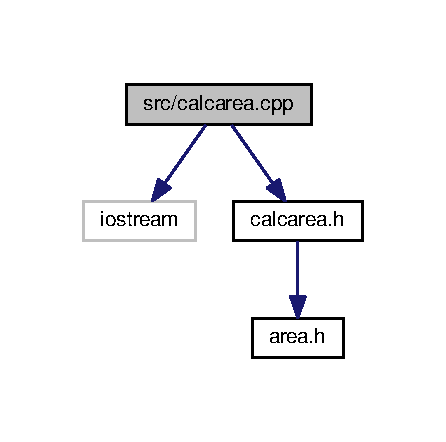
\includegraphics[width=214pt]{calcarea_8cpp__incl}
\end{center}
\end{figure}
\subsection*{Funções}
\begin{DoxyCompactItemize}
\item 
void \hyperlink{group__Figuras__Planas__Imprime__Area_gac0d6d9fb68ed0e43ad9780f0c86cac51}{calc\+Area\+Triangulo} (float \&base)
\begin{DoxyCompactList}\small\item\em Função que imprime o valor da área do triângulo. \end{DoxyCompactList}\item 
void \hyperlink{group__Figuras__Planas__Imprime__Area_ga1091311f26d5adb888dae930fc1ec7d6}{calc\+Area\+Retangulo} (float \&base, float \&altura)
\begin{DoxyCompactList}\small\item\em Função que imprime o valor da área do retângulo. \end{DoxyCompactList}\item 
void \hyperlink{group__Figuras__Planas__Imprime__Area_gaabb19ec0d92baa5524a15b463f854158}{calc\+Area\+Quadrado} (float \&base)
\begin{DoxyCompactList}\small\item\em Função que imprime o valor da área do quadrado. \end{DoxyCompactList}\item 
void \hyperlink{group__Figuras__Planas__Imprime__Area_gafc4965f40035f915dd29f3a2fe680339}{calc\+Area\+Circulo} (float \&raio)
\begin{DoxyCompactList}\small\item\em Função que imprime o valor da área do círculo. \end{DoxyCompactList}\item 
void \hyperlink{group__Figuras__Espaciais__Imprime__Area_gae484b707bcee07b0c5580440923326aa}{calc\+Area\+Piramide} (float \&base, float \&altura)
\begin{DoxyCompactList}\small\item\em Função que imprime o valor da área da pirâmide. \end{DoxyCompactList}\item 
void \hyperlink{group__Figuras__Espaciais__Imprime__Area_ga54aa7364c2caf59fa3d1b1b303901050}{calc\+Area\+Cubo} (float \&aresta)
\begin{DoxyCompactList}\small\item\em Função que imprime o valor da área do círculo. \end{DoxyCompactList}\item 
void \hyperlink{group__Figuras__Espaciais__Imprime__Area_ga153e7a3b91362f17f7f22919dde85ebc}{calc\+Area\+Paralelepipedo} (float \&aresta1, float \&aresta2, float \&aresta3)
\begin{DoxyCompactList}\small\item\em Função que imprime o valor da área do paralelepípedo. \end{DoxyCompactList}\item 
void \hyperlink{group__Figuras__Espaciais__Imprime__Area_ga3a49e8821532ada5f803c815f8d99825}{calc\+Area\+Esfera} (float \&raio)
\begin{DoxyCompactList}\small\item\em Função que imprime o valor da área do círculo. \end{DoxyCompactList}\end{DoxyCompactItemize}


\subsection{Descrição Detalhada}
Arquivo cabeçalho contendo a implementação das funções que solicitam ao usuário os dados necessários para o cálculo da área com a figura geométrica e chamam as funções que realizam essa operação. 

\begin{DoxyAuthor}{Autor}
Gabriel Barbosa (\href{mailto:gbsbarbosa.gb@gmail.com}{\tt gbsbarbosa.\+gb@gmail.\+com}) 

Ariel Oliveira (\href{mailto:ariel.oliveira01@gmail.com}{\tt ariel.\+oliveira01@gmail.\+com}) 
\end{DoxyAuthor}
\begin{DoxySince}{Desde}
09/03/2017 
\end{DoxySince}
\begin{DoxyDate}{Data}
12/03/2017 
\end{DoxyDate}
\begin{DoxySeeAlso}{Veja também}
\hyperlink{calcarea_8h}{calcarea.\+h} 
\end{DoxySeeAlso}

\hypertarget{calcperimetro_8cpp}{}\section{Referência do Arquivo src/calcperimetro.cpp}
\label{calcperimetro_8cpp}\index{src/calcperimetro.\+cpp@{src/calcperimetro.\+cpp}}


Arquivo de corpo contendo a implementacao das funções que solicitam ao usuário os dados necessários ao cálculo do perimetro da figura geométrica e chamam as funções que realizam essa operação.  


{\ttfamily \#include $<$iostream$>$}\\*
{\ttfamily \#include \char`\"{}calcperimetro.\+h\char`\"{}}\\*
Gráfico de dependência de inclusões para calcperimetro.\+cpp\+:
\nopagebreak
\begin{figure}[H]
\begin{center}
\leavevmode
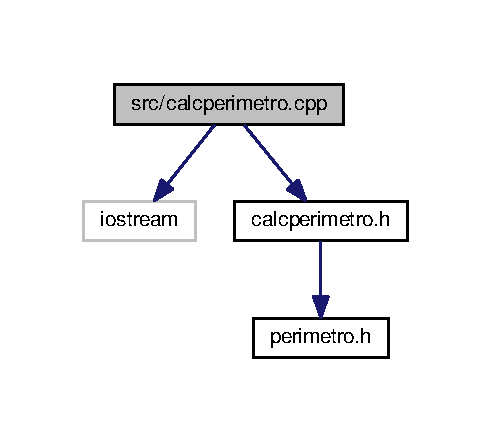
\includegraphics[width=236pt]{calcperimetro_8cpp__incl}
\end{center}
\end{figure}
\subsection*{Funções}
\begin{DoxyCompactItemize}
\item 
void \hyperlink{group__Figuras__Planas__Imprime__Perimetro_gae49d939eed738e7168cd0efd8b40c09c}{calc\+Perimetro\+Triangulo} (float \&base)
\begin{DoxyCompactList}\small\item\em Funcao que imprime o valor do perimetro do triangulo. \end{DoxyCompactList}\item 
void \hyperlink{group__Figuras__Planas__Imprime__Perimetro_gab29565d71c21097aef26e73d36b9c8a6}{calc\+Perimetro\+Retangulo} (float \&base, float \&altura)
\begin{DoxyCompactList}\small\item\em Funcao que imprime o valor do perimetro do retangulo. \end{DoxyCompactList}\item 
void \hyperlink{group__Figuras__Planas__Imprime__Perimetro_gacaef8cc731e8f6564e033dadcbefa04f}{calc\+Perimetro\+Quadrado} (float \&base)
\begin{DoxyCompactList}\small\item\em Funcao que imprime o valor do perimetro do quadrado. \end{DoxyCompactList}\item 
void \hyperlink{group__Figuras__Planas__Imprime__Perimetro_ga6f116584d476bf2a78f83cb668e1f25b}{calc\+Perimetro\+Circulo} (float \&raio)
\begin{DoxyCompactList}\small\item\em Funcao que imprime o valor do perimetro do circulo. \end{DoxyCompactList}\end{DoxyCompactItemize}


\subsection{Descrição Detalhada}
Arquivo de corpo contendo a implementacao das funções que solicitam ao usuário os dados necessários ao cálculo do perimetro da figura geométrica e chamam as funções que realizam essa operação. 

\begin{DoxyAuthor}{Autor}
Gabriel Barbosa (\href{mailto:gbsbarbosa.gb@gmail.com}{\tt gbsbarbosa.\+gb@gmail.\+com}) 

Ariel Oliveira (\href{mailto:ariel.oliveira01@gmail.com}{\tt ariel.\+oliveira01@gmail.\+com}) 
\end{DoxyAuthor}
\begin{DoxySince}{Desde}
09/03/2017 
\end{DoxySince}
\begin{DoxyDate}{Data}
12/03/2017 
\end{DoxyDate}
\begin{DoxySeeAlso}{Veja também}
\hyperlink{calcperimetro_8h}{calcperimetro.\+h} 
\end{DoxySeeAlso}

\hypertarget{calcvolume_8cpp}{}\section{Referência do Arquivo src/calcvolume.cpp}
\label{calcvolume_8cpp}\index{src/calcvolume.\+cpp@{src/calcvolume.\+cpp}}


Arquivo de corpo contendo a implementação das funções que solicitam ao usuário os dados necessários para o cálculo do volume com a figura geométrica e chamam as funções que realizam essa operação.  


{\ttfamily \#include $<$iostream$>$}\\*
{\ttfamily \#include \char`\"{}calcvolume.\+h\char`\"{}}\\*
Gráfico de dependência de inclusões para calcvolume.\+cpp\+:
\nopagebreak
\begin{figure}[H]
\begin{center}
\leavevmode
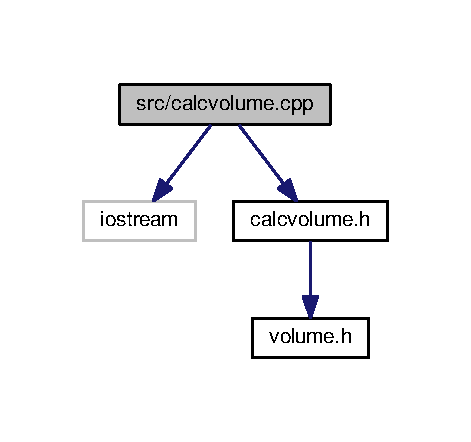
\includegraphics[width=226pt]{calcvolume_8cpp__incl}
\end{center}
\end{figure}
\subsection*{Funções}
\begin{DoxyCompactItemize}
\item 
void \hyperlink{group__Figuras__Espaciais__Imprime__Volume_gaa5acf0ff0f4eb8061d1b86334d2838de}{calc\+Volume\+Piramide} (float \&base, float \&altura)
\begin{DoxyCompactList}\small\item\em Função que imprime o valor do volume da pirâmide. \end{DoxyCompactList}\item 
void \hyperlink{group__Figuras__Espaciais__Imprime__Volume_gaf35d29634faa808e187b6635ac6e1fb9}{calc\+Volume\+Cubo} (float \&aresta)
\begin{DoxyCompactList}\small\item\em Função que imprime o valor do volume do cubo. \end{DoxyCompactList}\item 
void \hyperlink{group__Figuras__Espaciais__Imprime__Volume_ga994d3c26012b734a4cbabf0ce0c7b75b}{calc\+Volume\+Paralelepipedo} (float \&aresta1, float \&aresta2, float \&aresta3)
\begin{DoxyCompactList}\small\item\em Função que imprime o valor do volume do paralelepípedo. \end{DoxyCompactList}\item 
void \hyperlink{group__Figuras__Espaciais__Imprime__Volume_gaddef3fdcde1a2b12007610961caffae5}{calc\+Volume\+Esfera} (float \&raio)
\begin{DoxyCompactList}\small\item\em Função que imprime o valor do volume da esfera. \end{DoxyCompactList}\end{DoxyCompactItemize}


\subsection{Descrição Detalhada}
Arquivo de corpo contendo a implementação das funções que solicitam ao usuário os dados necessários para o cálculo do volume com a figura geométrica e chamam as funções que realizam essa operação. 

\begin{DoxyAuthor}{Autor}
Gabriel Barbosa (\href{mailto:gbsbarbosa.gb@gmail.com}{\tt gbsbarbosa.\+gb@gmail.\+com}) 

Ariel Oliveira (\href{mailto:ariel.oliveira01@gmail.com}{\tt ariel.\+oliveira01@gmail.\+com}) 
\end{DoxyAuthor}
\begin{DoxySince}{Desde}
09/03/2017 
\end{DoxySince}
\begin{DoxyDate}{Data}
12/03/2017 
\end{DoxyDate}
\begin{DoxySeeAlso}{Veja também}
\hyperlink{calcvolume_8h}{calcvolume.\+h} 
\end{DoxySeeAlso}

\hypertarget{main_8cpp}{}\section{src/main.cpp File Reference}
\label{main_8cpp}\index{src/main.\+cpp@{src/main.\+cpp}}


Programa que cálcula área, perímetro e volume de figuras geométricas planas e espaciais.  


{\ttfamily \#include $<$iostream$>$}\\*
{\ttfamily \#include $<$limits$>$}\\*
{\ttfamily \#include \char`\"{}calcarea.\+h\char`\"{}}\\*
{\ttfamily \#include \char`\"{}calcvolume.\+h\char`\"{}}\\*
{\ttfamily \#include \char`\"{}calcperimetro.\+h\char`\"{}}\\*
Include dependency graph for main.\+cpp\+:
% FIG 0
\subsection*{Functions}
\begin{DoxyCompactItemize}
\item 
void {\bfseries triangulo} ()\hypertarget{main_8cpp_a8928cef04d4cd48e92adf3569f6d185b}{}\label{main_8cpp_a8928cef04d4cd48e92adf3569f6d185b}

\item 
void {\bfseries retangulo} ()\hypertarget{main_8cpp_afa7da114af5845aed90385aaad07745f}{}\label{main_8cpp_afa7da114af5845aed90385aaad07745f}

\item 
void {\bfseries quadrado} ()\hypertarget{main_8cpp_a59a769deb5a89245b0b2a7760179708e}{}\label{main_8cpp_a59a769deb5a89245b0b2a7760179708e}

\item 
void {\bfseries circulo} ()\hypertarget{main_8cpp_a28482bc381ce414df86e4fdb9e3e6da5}{}\label{main_8cpp_a28482bc381ce414df86e4fdb9e3e6da5}

\item 
void {\bfseries piramide} ()\hypertarget{main_8cpp_ae3945922f925bc3d1fd95c5dc4ff6987}{}\label{main_8cpp_ae3945922f925bc3d1fd95c5dc4ff6987}

\item 
void {\bfseries cubo} ()\hypertarget{main_8cpp_af0b7d023166ce6902197d4082a66ad03}{}\label{main_8cpp_af0b7d023166ce6902197d4082a66ad03}

\item 
void {\bfseries paralelepipedo} ()\hypertarget{main_8cpp_af5c3350f35c2d9ae97c0243b7aeac39e}{}\label{main_8cpp_af5c3350f35c2d9ae97c0243b7aeac39e}

\item 
void {\bfseries esfera} ()\hypertarget{main_8cpp_a947bf2f326598c591bbdbf77a0280266}{}\label{main_8cpp_a947bf2f326598c591bbdbf77a0280266}

\item 
void {\bfseries menu} ()\hypertarget{main_8cpp_a2a0e843767aeea4f433a28b9c54f573a}{}\label{main_8cpp_a2a0e843767aeea4f433a28b9c54f573a}

\item 
void {\bfseries continua} (char $\ast$s)\hypertarget{main_8cpp_a5b6e29af98c7595c8ddf9771382fd141}{}\label{main_8cpp_a5b6e29af98c7595c8ddf9771382fd141}

\item 
void {\bfseries menu\+Escolha} (int escolha)\hypertarget{main_8cpp_a880038c883d20b974c3972ca68b2bdb0}{}\label{main_8cpp_a880038c883d20b974c3972ca68b2bdb0}

\item 
int {\bfseries main} ()\hypertarget{main_8cpp_ae66f6b31b5ad750f1fe042a706a4e3d4}{}\label{main_8cpp_ae66f6b31b5ad750f1fe042a706a4e3d4}

\end{DoxyCompactItemize}


\subsection{Detailed Description}
Programa que cálcula área, perímetro e volume de figuras geométricas planas e espaciais. 

Figuras geométricas planas possuem apenas área e perímetro, assim como as espaciais não possuem perímetro \begin{DoxyAuthor}{Author}
Gabriel Barbosa (\href{mailto:gbsbarbosa.gb@gmail.com}{\tt gbsbarbosa.\+gb@gmail.\+com}) 

Ariel Oliveira (\href{mailto:ariel.oliveira01@gmail.com}{\tt ariel.\+oliveira01@gmail.\+com}) 
\end{DoxyAuthor}
\begin{DoxySince}{Since}
09/03/2017 
\end{DoxySince}
\begin{DoxyDate}{Date}
12/03/2017 
\end{DoxyDate}

\hypertarget{perimetro_8cpp}{}\section{src/perimetro.cpp File Reference}
\label{perimetro_8cpp}\index{src/perimetro.\+cpp@{src/perimetro.\+cpp}}


Arquivo cabeçalho contendo a definição das funções que calculam o perímetro de figuras geométricas planas.  


{\ttfamily \#include \char`\"{}perimetro.\+h\char`\"{}}\\*
Include dependency graph for perimetro.\+cpp\+:
% FIG 0
\subsection*{Macros}
\begin{DoxyCompactItemize}
\item 
\#define {\bfseries PI}~3.\+1415\hypertarget{perimetro_8cpp_a598a3330b3c21701223ee0ca14316eca}{}\label{perimetro_8cpp_a598a3330b3c21701223ee0ca14316eca}

\end{DoxyCompactItemize}
\subsection*{Functions}
\begin{DoxyCompactItemize}
\item 
float \hyperlink{perimetro_8cpp_a76a18caf86cad87741930b6b73a28e6d}{triangulo\+Perimetro} (float \&base)
\begin{DoxyCompactList}\small\item\em Função que calcula o valor do perimetro do triângulo. \end{DoxyCompactList}\item 
float \hyperlink{perimetro_8cpp_a818dc286a8e9892293bddf8c2c4611dd}{retangulo\+Perimetro} (float \&base, float \&altura)
\begin{DoxyCompactList}\small\item\em Função que calcula o valor do perimetro do retângulo. \end{DoxyCompactList}\item 
float \hyperlink{perimetro_8cpp_a262504d9854cd41bc2519504de0531ca}{quadrado\+Perimetro} (float \&base)
\begin{DoxyCompactList}\small\item\em Função que calcula o valor do perímetro do quadrado. \end{DoxyCompactList}\item 
float \hyperlink{perimetro_8cpp_abf774992f344a535b77e941cabb7e2f0}{circulo\+Perimetro} (float \&raio)
\begin{DoxyCompactList}\small\item\em Função que calcula o valor do perimetro do círculo. \end{DoxyCompactList}\end{DoxyCompactItemize}


\subsection{Detailed Description}
Arquivo cabeçalho contendo a definição das funções que calculam o perímetro de figuras geométricas planas. 

\begin{DoxyAuthor}{Author}
Gabriel Barbosa (\href{mailto:gbsbarbosa.gb@gmail.com}{\tt gbsbarbosa.\+gb@gmail.\+com}) 

Ariel Oliveira (\href{mailto:ariel.oliveira01@gmail.com}{\tt ariel.\+oliveira01@gmail.\+com}) 
\end{DoxyAuthor}
\begin{DoxySince}{Since}
12/03/2017 
\end{DoxySince}
\begin{DoxyDate}{Date}
21/03/2017 
\end{DoxyDate}
\begin{DoxySeeAlso}{See also}
\hyperlink{perimetro_8h}{perimetro.\+h} 
\end{DoxySeeAlso}


\subsection{Function Documentation}
\index{perimetro.\+cpp@{perimetro.\+cpp}!circulo\+Perimetro@{circulo\+Perimetro}}
\index{circulo\+Perimetro@{circulo\+Perimetro}!perimetro.\+cpp@{perimetro.\+cpp}}
\subsubsection[{\texorpdfstring{circulo\+Perimetro(float \&raio)}{circuloPerimetro(float &raio)}}]{\setlength{\rightskip}{0pt plus 5cm}float circulo\+Perimetro (
\begin{DoxyParamCaption}
\item[{float \&}]{raio}
\end{DoxyParamCaption}
)}\hypertarget{perimetro_8cpp_abf774992f344a535b77e941cabb7e2f0}{}\label{perimetro_8cpp_abf774992f344a535b77e941cabb7e2f0}


Função que calcula o valor do perimetro do círculo. 

Funcao que calcula o valor do perimetro do circulo.


\begin{DoxyParams}{Parameters}
{\em raio} & R\+A\+IO valor da base do círculo \\
\hline
\end{DoxyParams}
\index{perimetro.\+cpp@{perimetro.\+cpp}!quadrado\+Perimetro@{quadrado\+Perimetro}}
\index{quadrado\+Perimetro@{quadrado\+Perimetro}!perimetro.\+cpp@{perimetro.\+cpp}}
\subsubsection[{\texorpdfstring{quadrado\+Perimetro(float \&base)}{quadradoPerimetro(float &base)}}]{\setlength{\rightskip}{0pt plus 5cm}float quadrado\+Perimetro (
\begin{DoxyParamCaption}
\item[{float \&}]{base}
\end{DoxyParamCaption}
)}\hypertarget{perimetro_8cpp_a262504d9854cd41bc2519504de0531ca}{}\label{perimetro_8cpp_a262504d9854cd41bc2519504de0531ca}


Função que calcula o valor do perímetro do quadrado. 

Funcao que calcula o valor do perimetro do quadrado.


\begin{DoxyParams}{Parameters}
{\em base} & B\+A\+SE valor da base do quadrado \\
\hline
\end{DoxyParams}
\index{perimetro.\+cpp@{perimetro.\+cpp}!retangulo\+Perimetro@{retangulo\+Perimetro}}
\index{retangulo\+Perimetro@{retangulo\+Perimetro}!perimetro.\+cpp@{perimetro.\+cpp}}
\subsubsection[{\texorpdfstring{retangulo\+Perimetro(float \&base, float \&altura)}{retanguloPerimetro(float &base, float &altura)}}]{\setlength{\rightskip}{0pt plus 5cm}float retangulo\+Perimetro (
\begin{DoxyParamCaption}
\item[{float \&}]{base, }
\item[{float \&}]{altura}
\end{DoxyParamCaption}
)}\hypertarget{perimetro_8cpp_a818dc286a8e9892293bddf8c2c4611dd}{}\label{perimetro_8cpp_a818dc286a8e9892293bddf8c2c4611dd}


Função que calcula o valor do perimetro do retângulo. 

Funcao que calcula o valor do perimetro do retangulo.


\begin{DoxyParams}{Parameters}
{\em base} & B\+A\+SE valor da base do retângulo \\
\hline
{\em altura} & A\+L\+T\+U\+RA valor da altura do retângulo \\
\hline
\end{DoxyParams}
\index{perimetro.\+cpp@{perimetro.\+cpp}!triangulo\+Perimetro@{triangulo\+Perimetro}}
\index{triangulo\+Perimetro@{triangulo\+Perimetro}!perimetro.\+cpp@{perimetro.\+cpp}}
\subsubsection[{\texorpdfstring{triangulo\+Perimetro(float \&base)}{trianguloPerimetro(float &base)}}]{\setlength{\rightskip}{0pt plus 5cm}float triangulo\+Perimetro (
\begin{DoxyParamCaption}
\item[{float \&}]{base}
\end{DoxyParamCaption}
)}\hypertarget{perimetro_8cpp_a76a18caf86cad87741930b6b73a28e6d}{}\label{perimetro_8cpp_a76a18caf86cad87741930b6b73a28e6d}


Função que calcula o valor do perimetro do triângulo. 

Função que calcula o valor do perimetro do triangulo.


\begin{DoxyParams}{Parameters}
{\em base} & B\+A\+SE valor da base do triangulo \\
\hline
\end{DoxyParams}

\hypertarget{volume_8cpp}{}\section{src/volume.cpp File Reference}
\label{volume_8cpp}\index{src/volume.\+cpp@{src/volume.\+cpp}}


Arquivo corpo contendo a Implementação das funções que calculam o volume de figuras geométricas espaciais.  


{\ttfamily \#include $<$cmath$>$}\\*
{\ttfamily \#include \char`\"{}volume.\+h\char`\"{}}\\*
Include dependency graph for volume.\+cpp\+:
\nopagebreak
\begin{figure}[H]
\begin{center}
\leavevmode
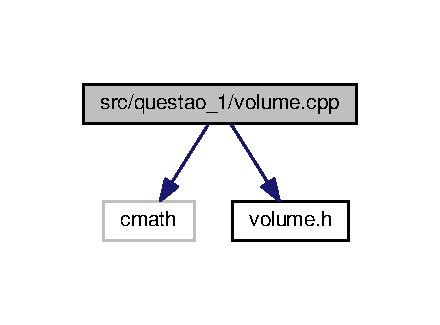
\includegraphics[width=198pt]{volume_8cpp__incl}
\end{center}
\end{figure}
\subsection*{Macros}
\begin{DoxyCompactItemize}
\item 
\#define {\bfseries PI}~3.\+1415\hypertarget{volume_8cpp_a598a3330b3c21701223ee0ca14316eca}{}\label{volume_8cpp_a598a3330b3c21701223ee0ca14316eca}

\end{DoxyCompactItemize}
\subsection*{Functions}
\begin{DoxyCompactItemize}
\item 
float \hyperlink{volume_8cpp_a4a36098bad980501fa8e5d0229309098}{volume\+Piramide} (float \&base, float \&altura)
\begin{DoxyCompactList}\small\item\em Funcao que calcula o valor do volume da piramide. \end{DoxyCompactList}\item 
float \hyperlink{volume_8cpp_a43aaef1a010e2ccbe7e5389aa5be3366}{volume\+Cubo} (float \&aresta)
\begin{DoxyCompactList}\small\item\em Funcao que calcula o valor do volume do cubo. \end{DoxyCompactList}\item 
float \hyperlink{volume_8cpp_adf67b3277ecfcf3e6e225e1f66e30a23}{volume\+Paralelepipedo} (float \&aresta1, float \&aresta2, float \&aresta3)
\begin{DoxyCompactList}\small\item\em Funcao que calcula o valor do volume do paralelepipedo. \end{DoxyCompactList}\item 
float \hyperlink{volume_8cpp_af649387c42d43094c7c81e2f26face42}{volume\+Esfera} (float \&raio)
\begin{DoxyCompactList}\small\item\em Funcao que calcula o valor do volume da esfera. \end{DoxyCompactList}\end{DoxyCompactItemize}


\subsection{Detailed Description}
Arquivo corpo contendo a Implementação das funções que calculam o volume de figuras geométricas espaciais. 

\begin{DoxyAuthor}{Author}
Gabriel Barbosa (\href{mailto:gbsbarbosa.gb@gmail.com}{\tt gbsbarbosa.\+gb@gmail.\+com}) 

Ariel Oliveira (\href{mailto:ariel.oliveira01@gmail.com}{\tt ariel.\+oliveira01@gmail.\+com}) 
\end{DoxyAuthor}
\begin{DoxySince}{Since}
09/03/2017 
\end{DoxySince}
\begin{DoxyDate}{Date}
12/03/2017 
\end{DoxyDate}
\begin{DoxySeeAlso}{See also}
\hyperlink{volume_8h}{volume.\+h} 
\end{DoxySeeAlso}


\subsection{Function Documentation}
\index{volume.\+cpp@{volume.\+cpp}!volume\+Cubo@{volume\+Cubo}}
\index{volume\+Cubo@{volume\+Cubo}!volume.\+cpp@{volume.\+cpp}}
\subsubsection[{\texorpdfstring{volume\+Cubo(float \&aresta)}{volumeCubo(float &aresta)}}]{\setlength{\rightskip}{0pt plus 5cm}float volume\+Cubo (
\begin{DoxyParamCaption}
\item[{float \&}]{aresta}
\end{DoxyParamCaption}
)}\hypertarget{volume_8cpp_a43aaef1a010e2ccbe7e5389aa5be3366}{}\label{volume_8cpp_a43aaef1a010e2ccbe7e5389aa5be3366}


Funcao que calcula o valor do volume do cubo. 


\begin{DoxyParams}{Parameters}
{\em aresta} & A\+R\+E\+S\+TA valor da aresta do cubo \\
\hline
\end{DoxyParams}
\begin{DoxyReturn}{Returns}
Volume do cubo 
\end{DoxyReturn}
\index{volume.\+cpp@{volume.\+cpp}!volume\+Esfera@{volume\+Esfera}}
\index{volume\+Esfera@{volume\+Esfera}!volume.\+cpp@{volume.\+cpp}}
\subsubsection[{\texorpdfstring{volume\+Esfera(float \&raio)}{volumeEsfera(float &raio)}}]{\setlength{\rightskip}{0pt plus 5cm}float volume\+Esfera (
\begin{DoxyParamCaption}
\item[{float \&}]{raio}
\end{DoxyParamCaption}
)}\hypertarget{volume_8cpp_af649387c42d43094c7c81e2f26face42}{}\label{volume_8cpp_af649387c42d43094c7c81e2f26face42}


Funcao que calcula o valor do volume da esfera. 


\begin{DoxyParams}{Parameters}
{\em raio} & R\+A\+IO valor do raio do cubo \\
\hline
\end{DoxyParams}
\begin{DoxyReturn}{Returns}
Volume da esfera 
\end{DoxyReturn}
\index{volume.\+cpp@{volume.\+cpp}!volume\+Paralelepipedo@{volume\+Paralelepipedo}}
\index{volume\+Paralelepipedo@{volume\+Paralelepipedo}!volume.\+cpp@{volume.\+cpp}}
\subsubsection[{\texorpdfstring{volume\+Paralelepipedo(float \&aresta1, float \&aresta2, float \&aresta3)}{volumeParalelepipedo(float &aresta1, float &aresta2, float &aresta3)}}]{\setlength{\rightskip}{0pt plus 5cm}float volume\+Paralelepipedo (
\begin{DoxyParamCaption}
\item[{float \&}]{aresta1, }
\item[{float \&}]{aresta2, }
\item[{float \&}]{aresta3}
\end{DoxyParamCaption}
)}\hypertarget{volume_8cpp_adf67b3277ecfcf3e6e225e1f66e30a23}{}\label{volume_8cpp_adf67b3277ecfcf3e6e225e1f66e30a23}


Funcao que calcula o valor do volume do paralelepipedo. 


\begin{DoxyParams}{Parameters}
{\em aresta1} & A\+R\+E\+S\+T\+A1 valor da aresta \#1 do paralelepipedo \\
\hline
{\em aresta2} & A\+R\+E\+S\+T\+A2 valor da aresta \#2 do paralelepipedo \\
\hline
{\em aresta3} & A\+R\+E\+S\+T\+A3 valor da aresta \#3 do paralelepipedo \\
\hline
\end{DoxyParams}
\begin{DoxyReturn}{Returns}
Valor do volume do paralelepipedo 
\end{DoxyReturn}
\index{volume.\+cpp@{volume.\+cpp}!volume\+Piramide@{volume\+Piramide}}
\index{volume\+Piramide@{volume\+Piramide}!volume.\+cpp@{volume.\+cpp}}
\subsubsection[{\texorpdfstring{volume\+Piramide(float \&base, float \&altura)}{volumePiramide(float &base, float &altura)}}]{\setlength{\rightskip}{0pt plus 5cm}float volume\+Piramide (
\begin{DoxyParamCaption}
\item[{float \&}]{base, }
\item[{float \&}]{altura}
\end{DoxyParamCaption}
)}\hypertarget{volume_8cpp_a4a36098bad980501fa8e5d0229309098}{}\label{volume_8cpp_a4a36098bad980501fa8e5d0229309098}


Funcao que calcula o valor do volume da piramide. 

Função que calcula o valor do volume da pirâmide.


\begin{DoxyParams}{Parameters}
{\em base} & B\+A\+SE valor da base da piramide \\
\hline
{\em altura} & A\+L\+T\+U\+RA valor da altura da piramide \\
\hline
\end{DoxyParams}
\begin{DoxyReturn}{Returns}
Volume da piramide 
\end{DoxyReturn}

%--- End generated contents ---

% Index
\backmatter
\newpage
\phantomsection
\clearemptydoublepage
\addcontentsline{toc}{chapter}{Index}
\printindex

\end{document}
